\documentclass[conference]{IEEEtran}
\IEEEoverridecommandlockouts
% The preceding line is only needed to identify funding in the first footnote. If that is unneeded, please comment it out.
\usepackage{cite}
\usepackage{amsmath,amssymb,amsfonts}
\usepackage{algorithmic}
\usepackage{graphicx}
\usepackage{textcomp}
\usepackage{xcolor}
\usepackage{xparse}
\NewDocumentCommand{\codeword}{v}{%
\texttt{\textcolor{blue}{#1}}%
}
\def\BibTeX{{\rm B\kern-.05em{\sc i\kern-.025em b}\kern-.08em
    T\kern-.1667em\lower.7ex\hbox{E}\kern-.125emX}}
\begin{document}

\title{Study Aid Tool - Group 27 BACK PACS \\
{\large Aiden Burgess - abur970 - 600280511}
}
\maketitle
\begin{abstract}

\end{abstract}

\section{Introduction}


\subsection{Motivation}
Students need to remove all distractions to study effectively. However, the process of setting up a relaxing environment for a session of focused work can be tedious and repetitive. Many students prefer to study with music in the background and with a nice wallpaper. When working on large problems or many problems, they like to break them down into smaller tasks in a todo list. It has become increasingly popular to use time-boxed techniques to maximise efficiency and focus, such as Pomodoro. Therefore, students may need to juggle many apps simultaneously, which can be distracting and annoying.

A unique feature that the team thought would be worthwhile to introduce is the ability to change the background and music based on the user's current mood.

\subsection{Goals}
The goals for this project were separated by priority into must-haves, should-haves, could-haves, and nice-to-haves. The list of proposed goals for the project can be found in Table 1.

As a summary, the main goals for the project was the mood-based functionality, which interacted with the background and music, and the todo list. These were chosen as the main goals because the unique feature of a mood.... The todo list is one of the most important components needed when a student is studying as it allows them to track their goals and progress for the study session.

With the same reasoning, white noise and a timer were should have functionality, as they aid a user's study.

\begin{table}[htbp]
\caption{Project Goals.}\label{tab1}
\resizebox{\columnwidth}{!}{\begin{tabular}{|p{18mm}|p{13mm}|p{45mm}|}
\cline{1-3} 
\textbf{\textit{Feature}}& \textbf{\textit{Time Estimate (Hours)}}& \textbf{\textit{Feature Description and Estimate Justification}} \\
\hline
\multicolumn{3}{|c|}{\textbf{Must-Haves}} \\
\hline
Mood based music player and recommendations & 20 & Get moods/preference from a mood slider and generate a playlist using the Spotify API that can be played in the browser. \\
\hline
Mood backgrounds & 12 & Generate some backgrounds based on the mood sliders/settings. Uses the splash API to retrieve backgrounds based on the search term. Create a slideshow with customisable interval. \\
\hline
Todo list & 10 & The ability to add items to a todo list which can help the user keep track of their progress.
Does not use third-party tools. \\
\hline
\multicolumn{3}{|c|}{\textbf{Should-Haves}} \\
\hline
White noise & 8 & A feature that will generate white noise for the user to aid in their study.
Simple white noise audio file that can play/pause. Reuse styling from the music recommender above. \\
\hline
Timer & 6 & A timer that can countdown and allow the user to keep track of time and perhaps implement study strategies like Pomodoro. \\
\hline
\multicolumn{3}{|c|}{\textbf{Could-Haves}} \\
\hline
Whiteboard & 8 & A whiteboard that the user can use to draw and save some of the images to help with their study. 
Use Third party components. \\
\hline
Study statistics & 15 & Statistics that summarise the user’s music time, study time, items added and completed. This can be used to help the student with seeing how much progress they are making. \\
\hline
User accounts & 20 & User accounts which remember the user’s preferences, with login details, and the ability to access preferences from multiple accounts.
Using a database over local storage. \\
\hline
\multicolumn{3}{|c|}{\textbf{Nice-To-Haves}} \\
\hline 
Music recommendations based on weather & 10 & Get the user location, and weather, then give a music recommendation using the Music Player already implemented. \\
\hline
Inspirational messages & 5 & Generating inspirational messages using API to display. \\
\hline
\end{tabular}}
\end{table}


\section{Related Work}
%What has been done before? Compare it with your project.

%BELOW IS ALL COPIED, NEED TO CHANGE AND MERGE WITH PRESENTATION

The preliminary market research revealed that no app exists with all the proposed app’s functionality. However, some apps/services exist which partially provide one of the features from our proposed feature-set. Below is a discussion on other apps which offer our top three features.

Spotify provides in-app music recommendations based on the user’s song history. Besides individual songs, Spotify recommends playlists which we will reproduce in our app. However, Spotify does not have any mood sliders based on which the current queue of songs. This is a feature which we will add to our app. 

The ‘mood backgrounds’ feature is something that no app currently offers. However, an app called ‘MoodTurn’ allows the user to choose a background category such as ‘beach’ or ‘nature’, then starts a background slideshow whilst playing soothing music associated with the pictures. We aim to keep the slideshow feature from this app, but instead of picture categories, we will have a way to change the pictures dynamically based on the user’s mood. 

Todoist is a comprehensive app that allows the user to create todo lists. It has a plethora of features, such as creating recurring events and delegating tasks to other people. While we will keep some basic features of this app, such as arranging the tasks date-wise, we do not aim to include the other complex features in our app.


\section{Design}
%Software architecture (e.g. class diagram)? User interface (e.g. screen diagram)? Why this design?

\subsection{Visual Design}
The visual design process began with an ideation phase, where each team member came up with some ideas for the overall design of the app. Some ideas were to have the components as widgets floating on the screen, hacing a grid with the components fixed in place, having the components in tabs, and having a main menu to reach the components. 

From this, each of the ideas was ranked by each team member, and the idea with the highest rank was chosen, which was to have the copmonents as widgets floating on the screen.

After this phase, we collaborated on Mural to produce lo-fi prototypes for some of the components and screens (Fig \ref{prototyping}.)

\begin{figure}[htbp]
\centerline{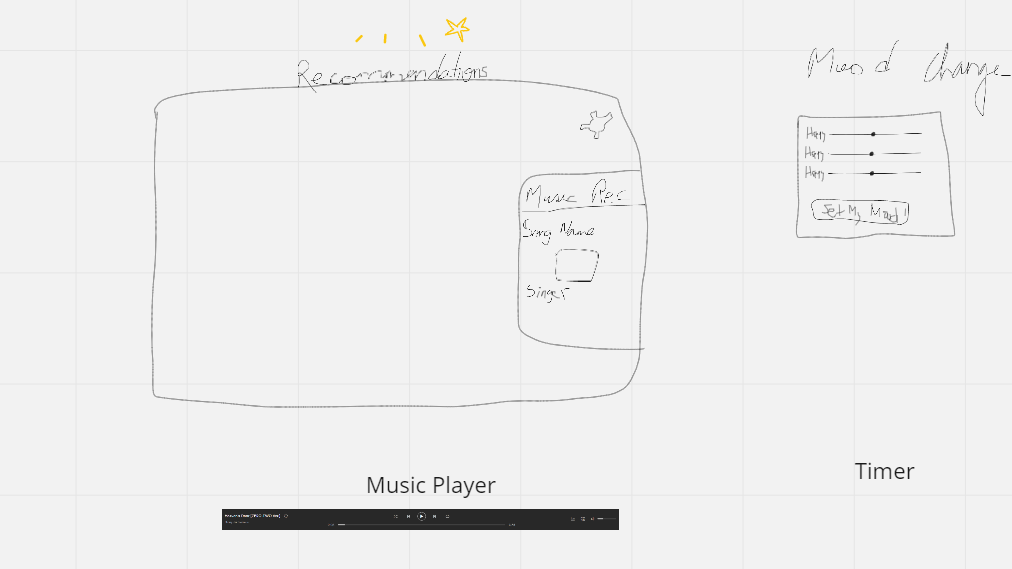
\includegraphics[width = \linewidth]{prototyping.png}}
\caption{Lo-fi prototyping process.}
\label{prototyping}
\end{figure}

\subsection{Architectural Design}
An overview of our design for the system architecture can be found in Figure \ref{project-architecture}. It follows a common industry pattern of a frontend, which is connected to the backend, and a backend connected to the database. This pattern ensures that user requests are validated and authorised by the backend before reaching the database, improving security and reducing complexity and processing in the frontend.


\begin{figure}[htbp]
\centerline{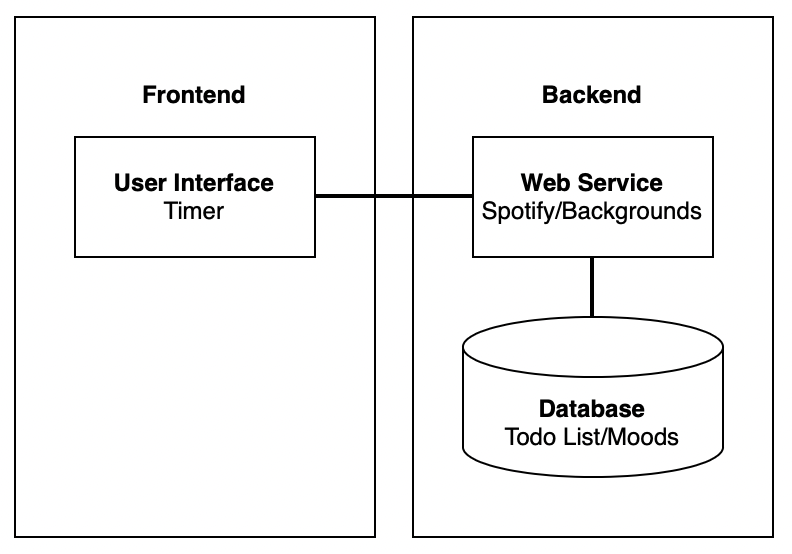
\includegraphics[width = \linewidth]{project-architecture.png}}
\caption{Project architecture.}
\label{project-architecture}
\end{figure}

The frontend is responsible for serving the website interface to users. It retrieves data from the backend, and displays it to the user. It also handles the logic of the website, such as inputs for the mood, playing a slideshow of backgrounds, and playing music. The timer component is purely in the frontend as there is no data or external apis associated with it.

The backend of this application has two main functions. Firstly, it validates, authorises and executes user queries on the database, such as changing the mood or adding a todo item. This is the use case for the mood component and the todo component. Secondly, it handles interactions with other external apis and preprocesses the data to return to the user. This function is used for the music API and background API.

The database role and schema is relatively simple. It stores the mood and todo list data per session. Each session can either belong to a user, or to a guest. There is no storage needed for the music, timer or background components.

%api routes split
%What did the backend do
%what did the database store, what did it not store
%Frontend split up into independent components
%How was state managed?

\section{Implementation}
%What have we implemented? 
%Technologies?
%How was the work split up
%Split into team contribution and individual?

Note: In this section I will talk solely about my individual contributions to the project.

From the project roadmap (Fig \ref{roadmap}.), we can see there are seven main epics for the project. I worked on the mood slider and timer components. The mood slider also required integration with the spotify and background components. I also developed the login page of the application and styling for my components.

\begin{figure}[htbp]
\centerline{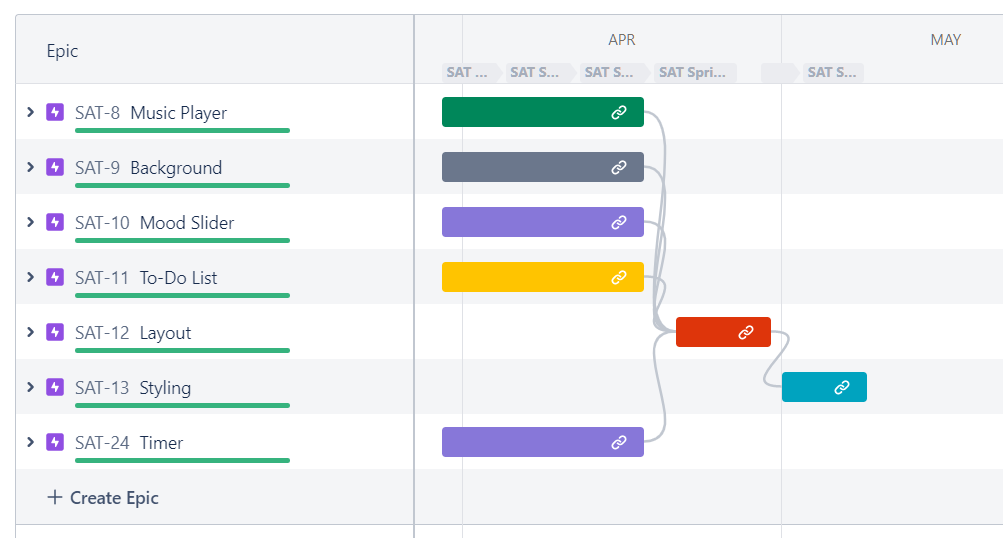
\includegraphics[width = \linewidth]{project-roadmap.png}}
\caption{Project roadmap.}
\label{roadmap}
\end{figure}

\subsection{Timer}
The simplest and first component that I implemented is the timer component (top left Fig \ref{homepage}.). It does not require any backend or database interaction, as it is a purely frontend component. I started by using an existing component I found online for the timer component. Then, I added a validated user input to specify the time requested, and the buttons for starting and stopping the timer.

\subsection{Mood Slider}
Next was the mood slider (bottom left Fig \ref{homepage}.). The frontend of the mood component was again started from an existing component I found online. This required a database to store the moods per user, so I created a MongoDB Cloud database for the project. The schema for the mood was a nested mood object consisting of five fields inside a larger user object. The backend code was located in the route \codeword{api/mood}. I also implemented the backend testing for the overall user route, which contained the functionality for moods and todo lists.

Finally, the mood needed to be integrated with the background and music components. The mood was stored in the application globally and the \codeword{useEffect()} function was used to react to changes in this state. When the mood changes, the background and spotify components both update. The background component has more complex functionality as there is no direct way to map the mood to a background. Therefore, a \codeword{moodToSearchParser} was developed acting as a translator. For example, if valence is high then the term "happy" is added to the search terms used to find backgrounds.

\begin{figure}[htbp]
\centerline{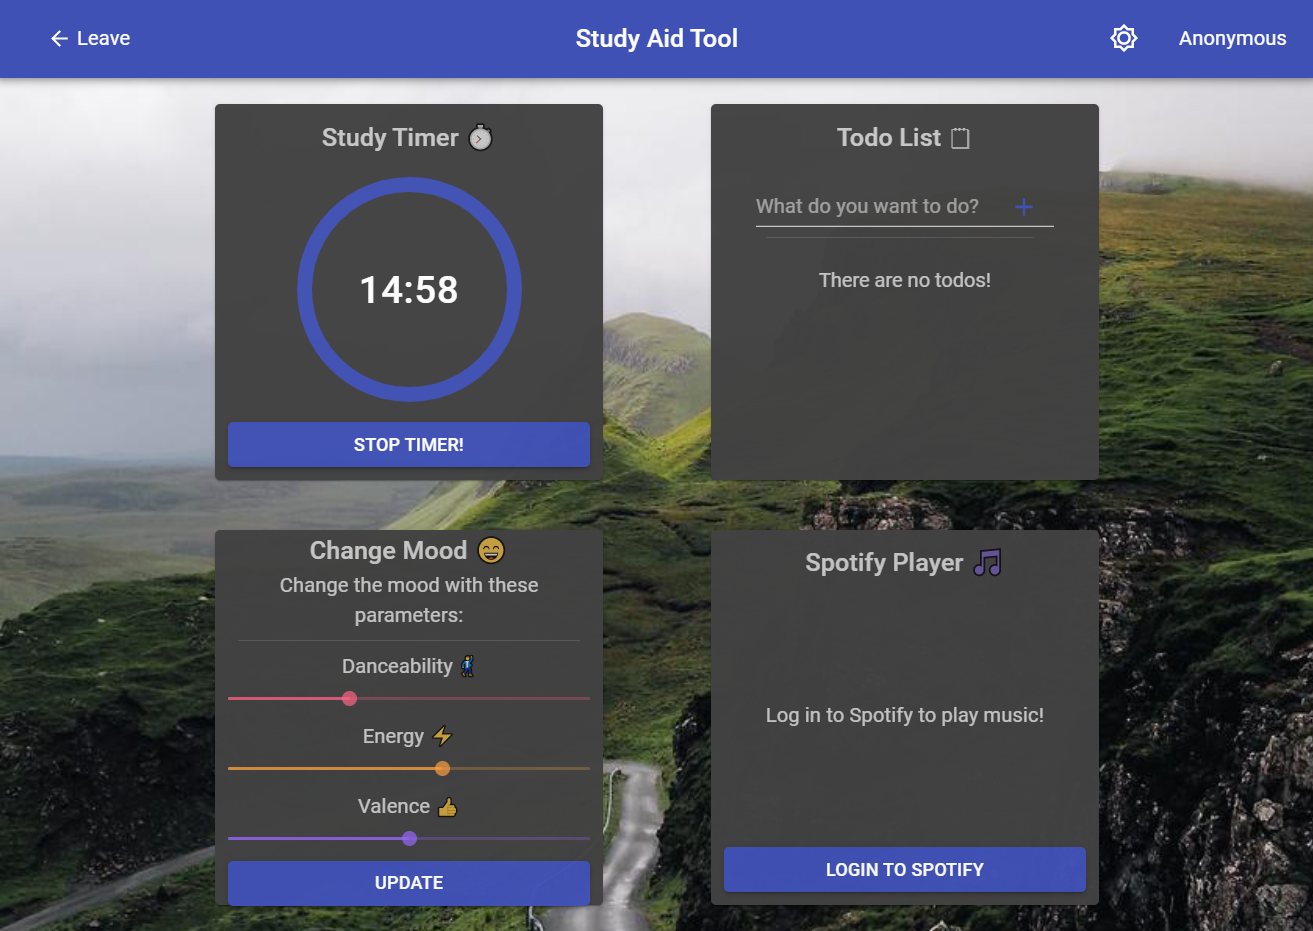
\includegraphics[width = \linewidth]{homepage.png}}
\caption{Application homepage.}
\label{homepage}
\end{figure}

\subsection{Sign-in Page}
Near the end of the project, I was assigned with styling the homepage, as it was empty with two buttons. From some quick research I found that the login and sign buttons were often offset on a homepage, so I designed the homepage following this pattern (Fig \ref{signin}.). Originally I used a static image, but I found that a GIF with a starfield animation was more engaging. The GIF used is a well known meme around studying called the lofi girl.

\begin{figure}[htbp]
\centerline{\includegraphics[width = \linewidth]{signin.png}}
\caption{Application sign in page.}
\label{signin}
\end{figure}

\section{Testing}
Our application has tests for both the frontend and backend systems.

Shallow and snapshot testing was performed on the frontend. Shallow testing is rendering a single component and asserting its behaviour. It allows us to check that the component is loaded correctly while ignoring the implementation of the children elements. "A [sic] snapshot test renders a UI component, takes a snapshot, then compares it to a reference snapshot file stored alongside the test.\cite{b1}" It ensures that no unexpected changes occur between versions.

Backend testing was performed via Jest and mocks. As our project relies heavily on external APIs, we had to mock these services when writing unit tests for the application. This decouples the correctness of our application from the correctness of the APIs we use. We used an in-memory mongodb server to reduce coupling between the backend and database, and to improve test speed.

\section{Methodology}
Our team followed an Agile process, with one team leader (Sam), and two team meetings per week. We also utilised many technologies such as Jira, GitHub, and Discord to manage our project.

\subsection{Technologies}
\subsubsection{Jira}
Jira is a product by Atlassian to manage a project's tickets and progress (Fig \ref{progress}.). We utilised it heavily to track what tasks team members were assigned, and to manage our weekly sprints. Jira has a built-in sprint board, and backlog which synergized with our Agile approach.

\subsubsection{Github}
We utilised GitHub as our version control system of choice. A new branch was created on GitHub for each ticket on Jira. The naming convention of the branches included the ticket id and the feature, for example \codeword{AnubhavKhanna07/SAT-84/timer-colour-dark-mode}. This allowed tickets to be tracked more easily. After the feature was implemented, a pull request was made against the main branch and at least one other member commented or approved the request (Fig \ref{github}.). GitHub Actions was also utilised to automatically run the frontend and backend tests on each pull request. 

\begin{figure}[htbp]
\centerline{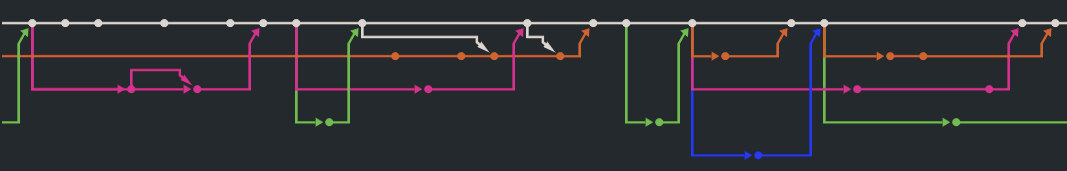
\includegraphics[width = \linewidth]{github-network.png}}
\caption{GitHub network map.}
\label{github}
\end{figure}

\subsubsection{Discord}
Discord is a messaging application with built in voice channels, video streaming, and screen-sharing. We used it in this project for most of our communication, and for video calls. I also integrated it with GitHub so that each action on the repository such as test results and pull requests was shown in Discord.

\subsubsection{Messenger}
Messenger is Facebook's messaging platform, which focuses on more real-time interaction. As each team member used Facebook, we would be notified immediately about new messages, so this was used for more timely discussions and reminders (Fig \ref{messenger}.). There is only a single channel, which makes it difficult to manage multiple conversations and topics, so Discord was used in conjunction with Messenger.

\begin{figure}[htbp]
\centerline{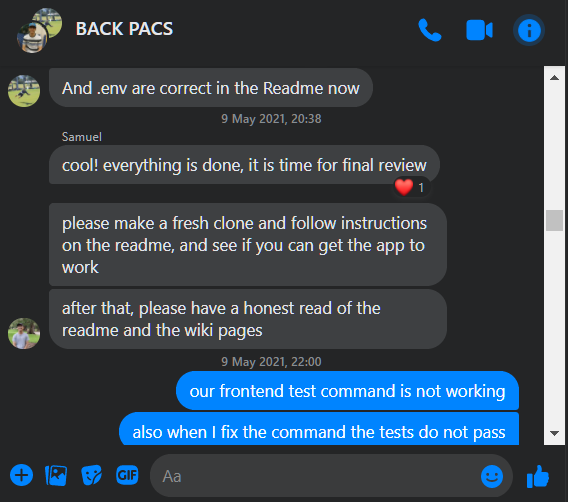
\includegraphics[width = \linewidth]{messenger.png}}
\caption{Example Messenger messages.}
\label{messenger}
\end{figure}

\subsection{Agile}
%Can add a screenshot of burndown
The Agile methodology is a software development process which focuses on iterative development and fast iterations \cite{b2}. Out team held one-week long sprints, and Jira helped track these. The sprints started on Monday, and we held a mid-sprint review on Thursdays to check if anyone had any significant blockers or interesting things to report.

On Monday, we reviewed the sprint, and work was assigned to each team member. During this session we discussed what had been completed and what we could do in the next week. 

From the progress chart \ref{progress}, we can see that there is constant progress on the application every week, with the jumps in "To Do" occuring each Monday as tasks were assigned. As the deadline approached, the workload seems to increase, as smaller tickets such as bugfixes are added.

\begin{figure}[htbp]
\centerline{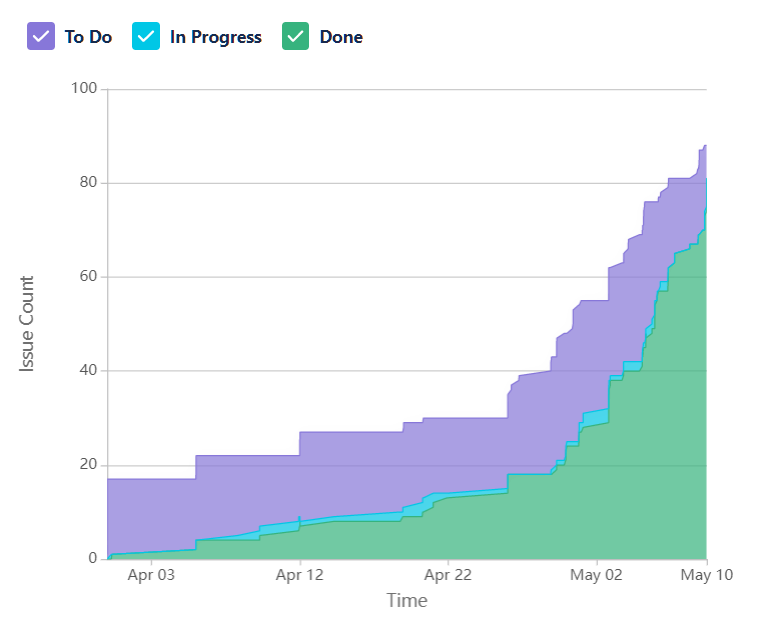
\includegraphics[width = \linewidth]{cumulative-flow-diagram.png}}
\caption{Cumulative progress chart.}
\label{progress}
\end{figure}

\section{Discussion}
\subsection{Progress on Goals}
Our team implemented all of the must-haves, two of the should-haves, and one of the could-haves. 

Along with these goals that were specified at the beginning of the project, other smaller features were also added to the system. A homepage was added which was not originally in the design


\subsection{Challenges}
% This part needs to be rewritten
One of the challenges we faced was that Sam was in Australia for the first 7 weeks of the project, so we had to hold our meetings online via Discord and Zoom

Another challenge was working with the spotify player api, as many teams have discussed previously, there are some frustrating parts of the spotify api, such as needing spotify premium to play music through spotify player api, and authentication protocols were proprietary and difficult to learn


\section{Conclusion}
%Conclusions? Lessons? Future work?


\section*{Acknowledgment}

\section*{References}

%For papers published in translation journals, please give the English 
%citation first, followed by the original foreign-language citation \cite{b6}.

\begin{thebibliography}{00}
\bibitem{b1}"Snapshot Testing · Jest", Jestjs.io, 2021. [Online]. Available: https://jestjs.io/docs/snapshot-testing. [Accessed: 09- Jun- 2021].
\bibitem{b2}"What is AGILE? - What is SCRUM? - Agile FAQ's | Cprime", Cprime, 2021. [Online]. Available: https://www.cprime.com/resources/what-is-agile-what-is-scrum/. [Accessed: 09- Jun- 2021].
\end{thebibliography}


\end{document}
